\documentclass[UTF8,zihao=-4,a4paper]{ctexart}
\usepackage[a4paper,margin=2.35cm,headheight=14pt]{geometry}
\usepackage{amsmath,amssymb,booktabs,graphicx,float,hyperref,xcolor,fancyhdr,enumitem,lastpage}
\setCJKmainfont{Noto Serif CJK SC}
\setCJKsansfont{Noto Sans CJK SC}
\setmainfont{Liberation Serif}
\definecolor{titlec}{HTML}{22476A}
\hypersetup{colorlinks=true,linkcolor=titlec,urlcolor=titlec,
  pdftitle={DANDI 000138: source-only fixed KMeans groups and Hard HiWA}}
\graphicspath{{results/source_only_fixed_groups/}}
\pagestyle{fancy}\fancyhf{}
\fancyhead[L]{\footnotesize DANDI 000138 · 单次源域硬分组实验}
\fancyhead[R]{\footnotesize 2026-11-17}
\fancyfoot[C]{\thepage\ /\pageref{LastPage}}
\makeatletter\let\primitiveinput\@@input\makeatother
\newcommand{\R}{\mathbb{R}}
\begin{document}

\begin{center}
{\Huge\bfseries\color{titlec}四维 Hard HiWA 实验 C}\\[7pt]
{\LARGE 仅源域 K-means，唯一标签贯穿对齐前后}\\[14pt]
{\small 正式重做报告 · 真实 DANDI 数据 · 原版 PyHiWA · 可复现}\\
\end{center}
\noindent\rule{\linewidth}{0.6pt}

\section{为什么重新做实验}
先前的实验在神经域与手部运动域\emph{分别}执行 K-means，
所得标签不具备统一的组意义；用相同颜色比较两个域因此可能误导。
本次\textbf{不独立聚类目标域}，改为在神经源域执行\emph{唯一的一次 K-means}，
通过同步试次与时窗的一一对应把源标签传给目标。
旋转或最优传输后\textbf{不改变任何点的簇标签}。

\noindent\fbox{\parbox{0.94\linewidth}{\small\textbf{重要方法学声明：}
虽然 HiWA 求解器的实例级 Sinkhorn 仍不直接使用一对一样本配对，
但目标域标签是通过已知神经--手部同步配对复制来的；
因此\emph{分组层面使用了对应监督信息}，本次并非完全无监督、无配对的对齐实验。
不得把结果与之前的独立聚类基线当作只改了一个超参数的消融。}}

\section{数据集与预处理}
来自 \href{https://dandiarchive.org/dandiset/000138/0.220113.0407}
{DANDI:000138, MC\_Maze\_Large, v0.220113.0407}：
记录猕猴延迟伸手任务中的运动皮层放电和手部位置/速度。
输入来自同一份可复现的官方 NWB 派生四维缓存，使用
500 个有效试次，其中 400 个训练、100 个留出测试，
每试次相对 \texttt{move\_onset\_time} 的
$[-100,600]$\,ms 以 20\,ms 间隔采样，得到
$14000$ 训练窗口和 $3500$ 测试窗口。

源域：162 个神经单元的 spike count/20\,ms$\to$平方根变换
$\to$40\,ms Gaussian 平滑$\to$训练集通道标准化$\to$PCA(4)，得到
$X\in\R^{17500\times4}$。
目标域直接保留
$Y=(p_x,p_y,v_x,v_y)\in\R^{17500\times4}$，
只用训练集统计量标准化，\textbf{没有 PCA}。
两域在求解器输入时各自减去训练均值、除以单一训练 RMS 半径。
之前数据中的\emph{目标域旧 K-means 标签完全不被本实验使用}。

\section{一次聚类、继承标签与原版硬对齐}
只在源域训练样本上拟合：
\begin{equation}
 g=\operatorname{KMeans}(X_{\mathrm{train}};\,K=4,
 \texttt{n\_init}=20,\texttt{seed}=42),\qquad
 c_i=g(x_i).
\end{equation}
固定同步索引 $i$，并令
\begin{equation}
 \boxed{\operatorname{group}_X(x_i)=
        \operatorname{group}_Y(y_i)=c_i,\quad
        \operatorname{group}_{\widehat RX}(\widehat R x_i)=c_i.}
\end{equation}
对测试源域仅用训练拟合的 $g$ 预测标签，再复制给对应目标测试样本。
这一过程没有 K-means($Y$)，也没有 K-means($\widehat RX$)。

使用上传压缩包内的原版 \texttt{hiwa\_original.py}，
以完全相同的源/目标组标签运行 Hard HiWA。
求解过程包括局部最优传输、簇间 Sinkhorn、全局正交矩阵
$\widehat R\in O(4)$ 的 ADMM 更新，
\textbf{不修改原版算法}。外循环最多 140 次，
$\mu=0.05$，组间 Sinkhorn $\gamma=0.2$、200 次，
实例级 $\gamma=0.1$、45 次，局部最多 20 次，
每个域从每簇独立随机抽取 40 个窗口。
分别运行种子 42、43、44、45、46。
\textbf{可视化预注册 seed 42，不根据测试指标择优挑图}。

\section{固定组的四维源--目标散点图}
以下所有图使用\textbf{同一批留出测试窗口}、同一组继承标签、
同一四维坐标规范化和\textbf{每个对应投影完全相同的坐标轴范围}。
每张图显示 $\binom42=6$ 个二维坐标投影；聚类始终在四维完成。

\begin{figure}[p]\centering
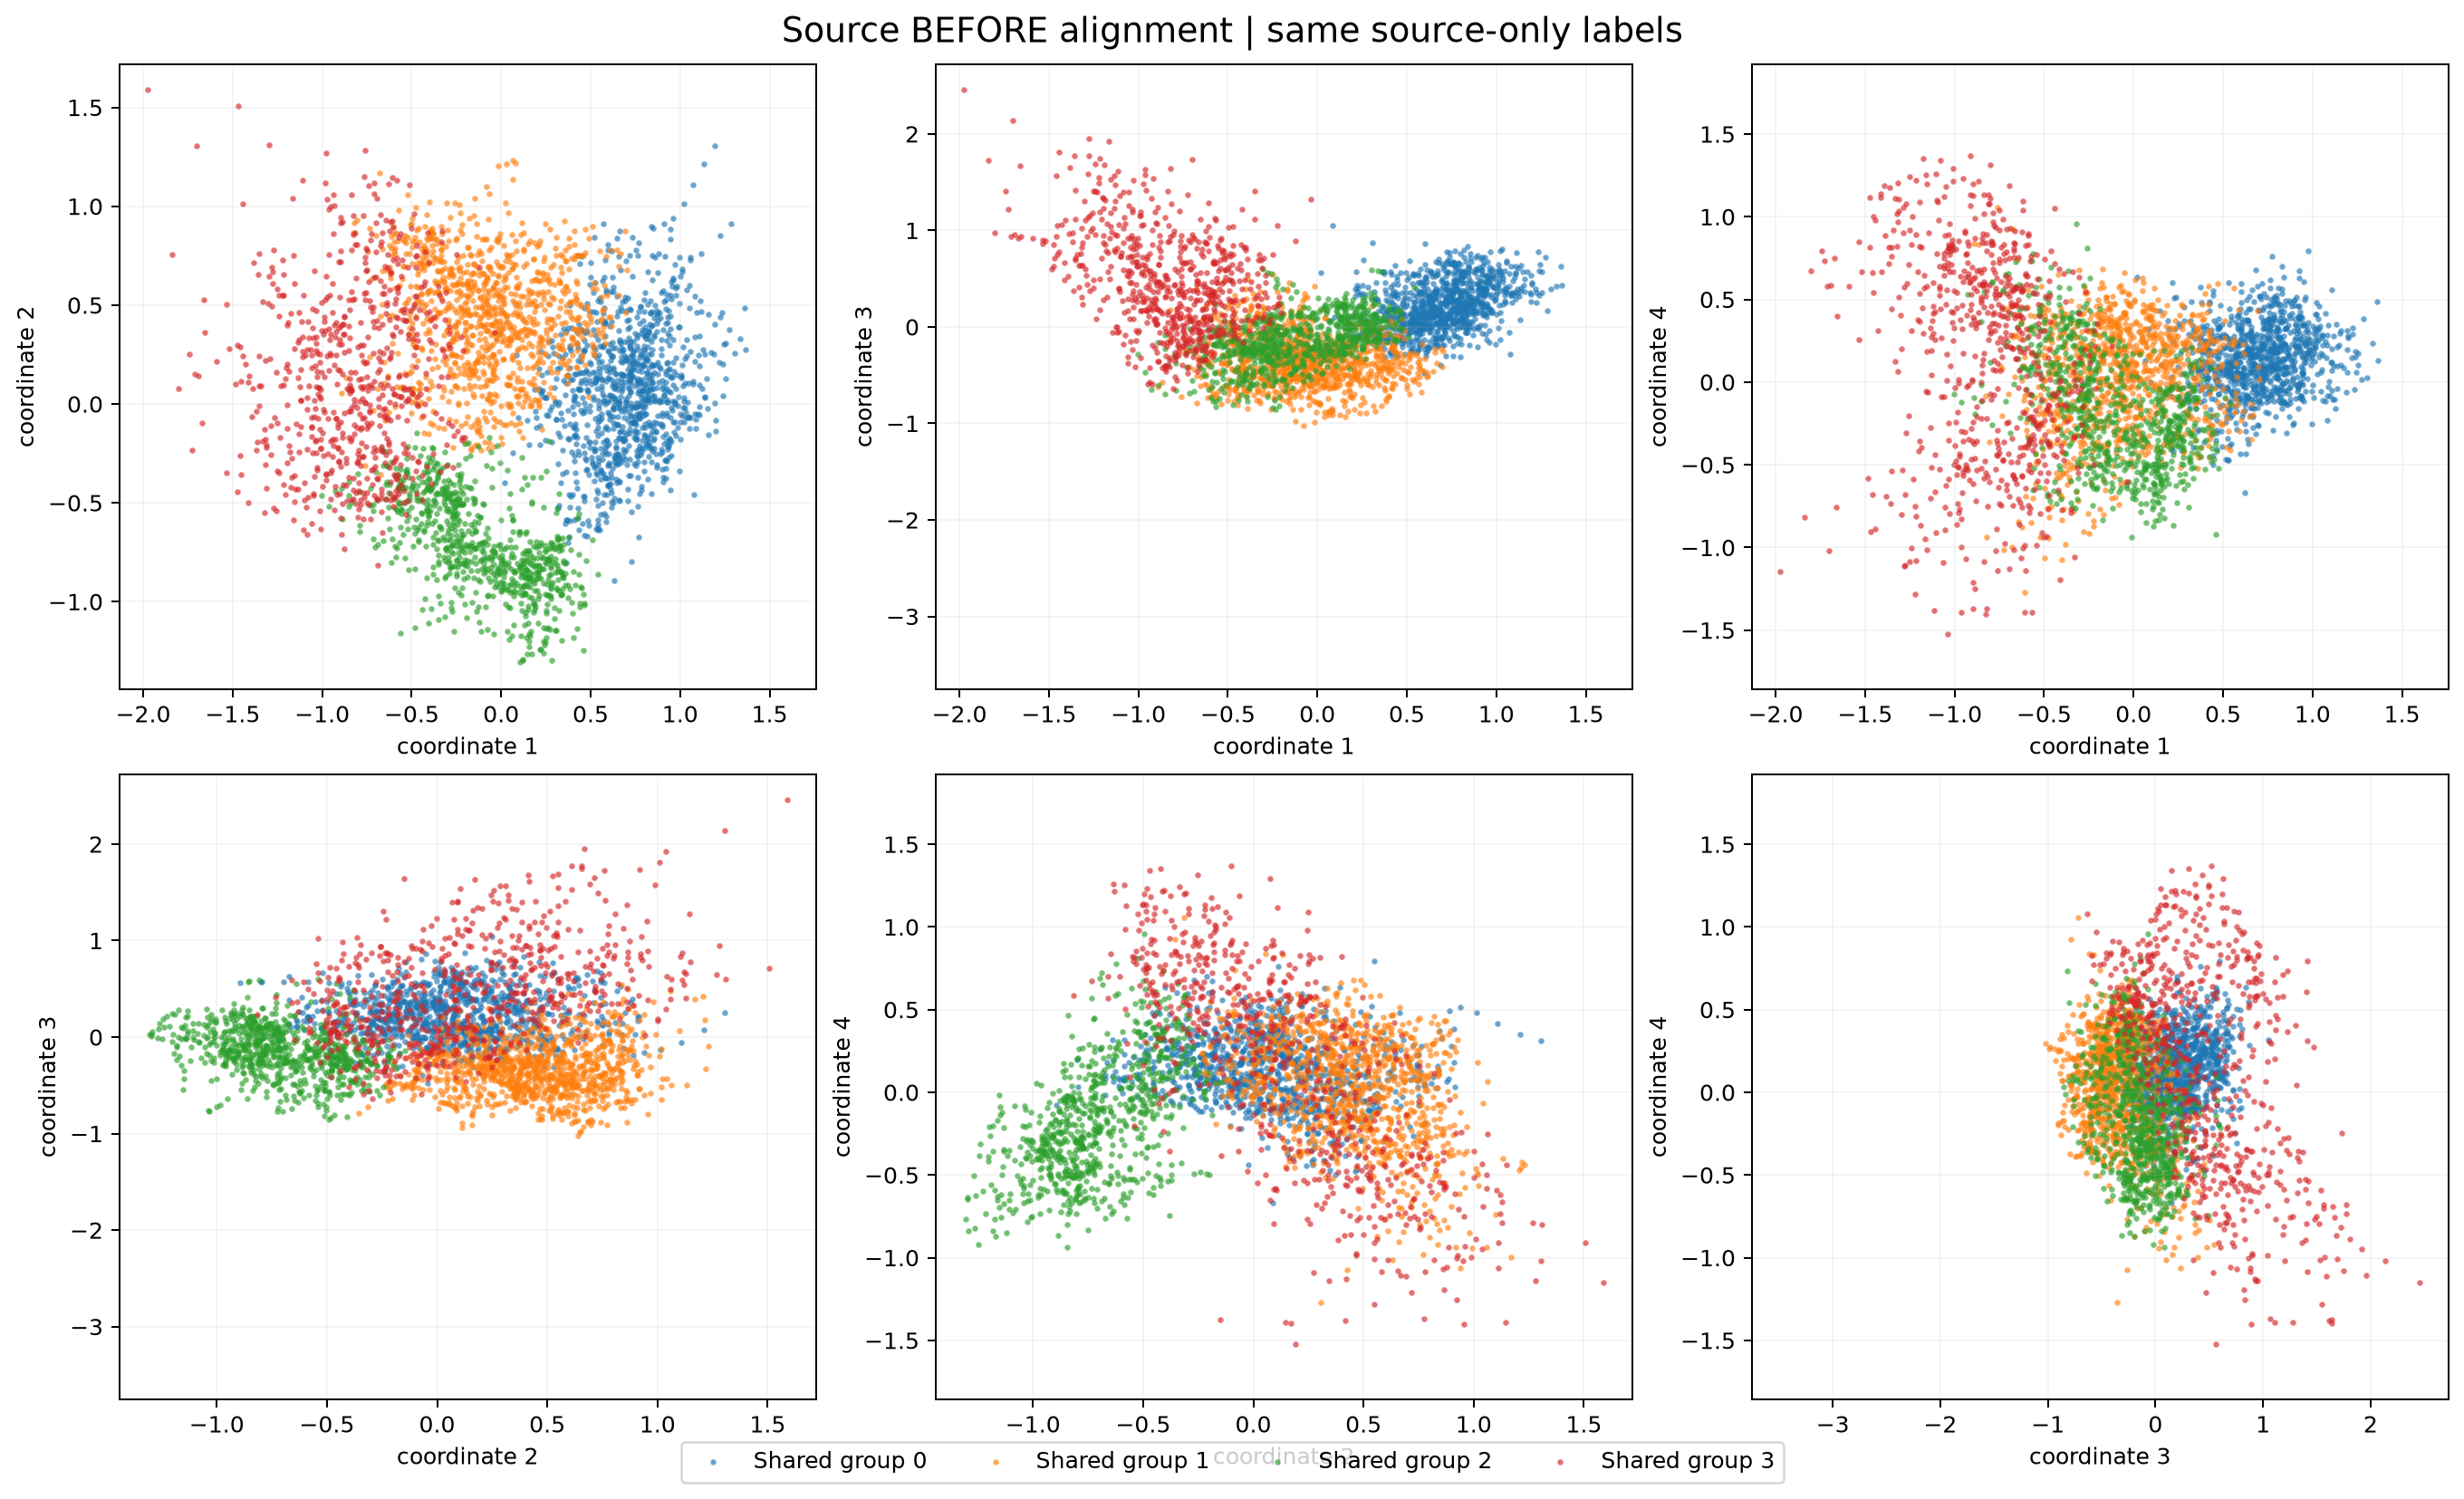
\includegraphics[width=\textwidth]{source_before_test_six.png}
\caption{对齐前神经源域：唯一源域 K-means 的固定标签。}
\end{figure}
\clearpage
\begin{figure}[p]\centering
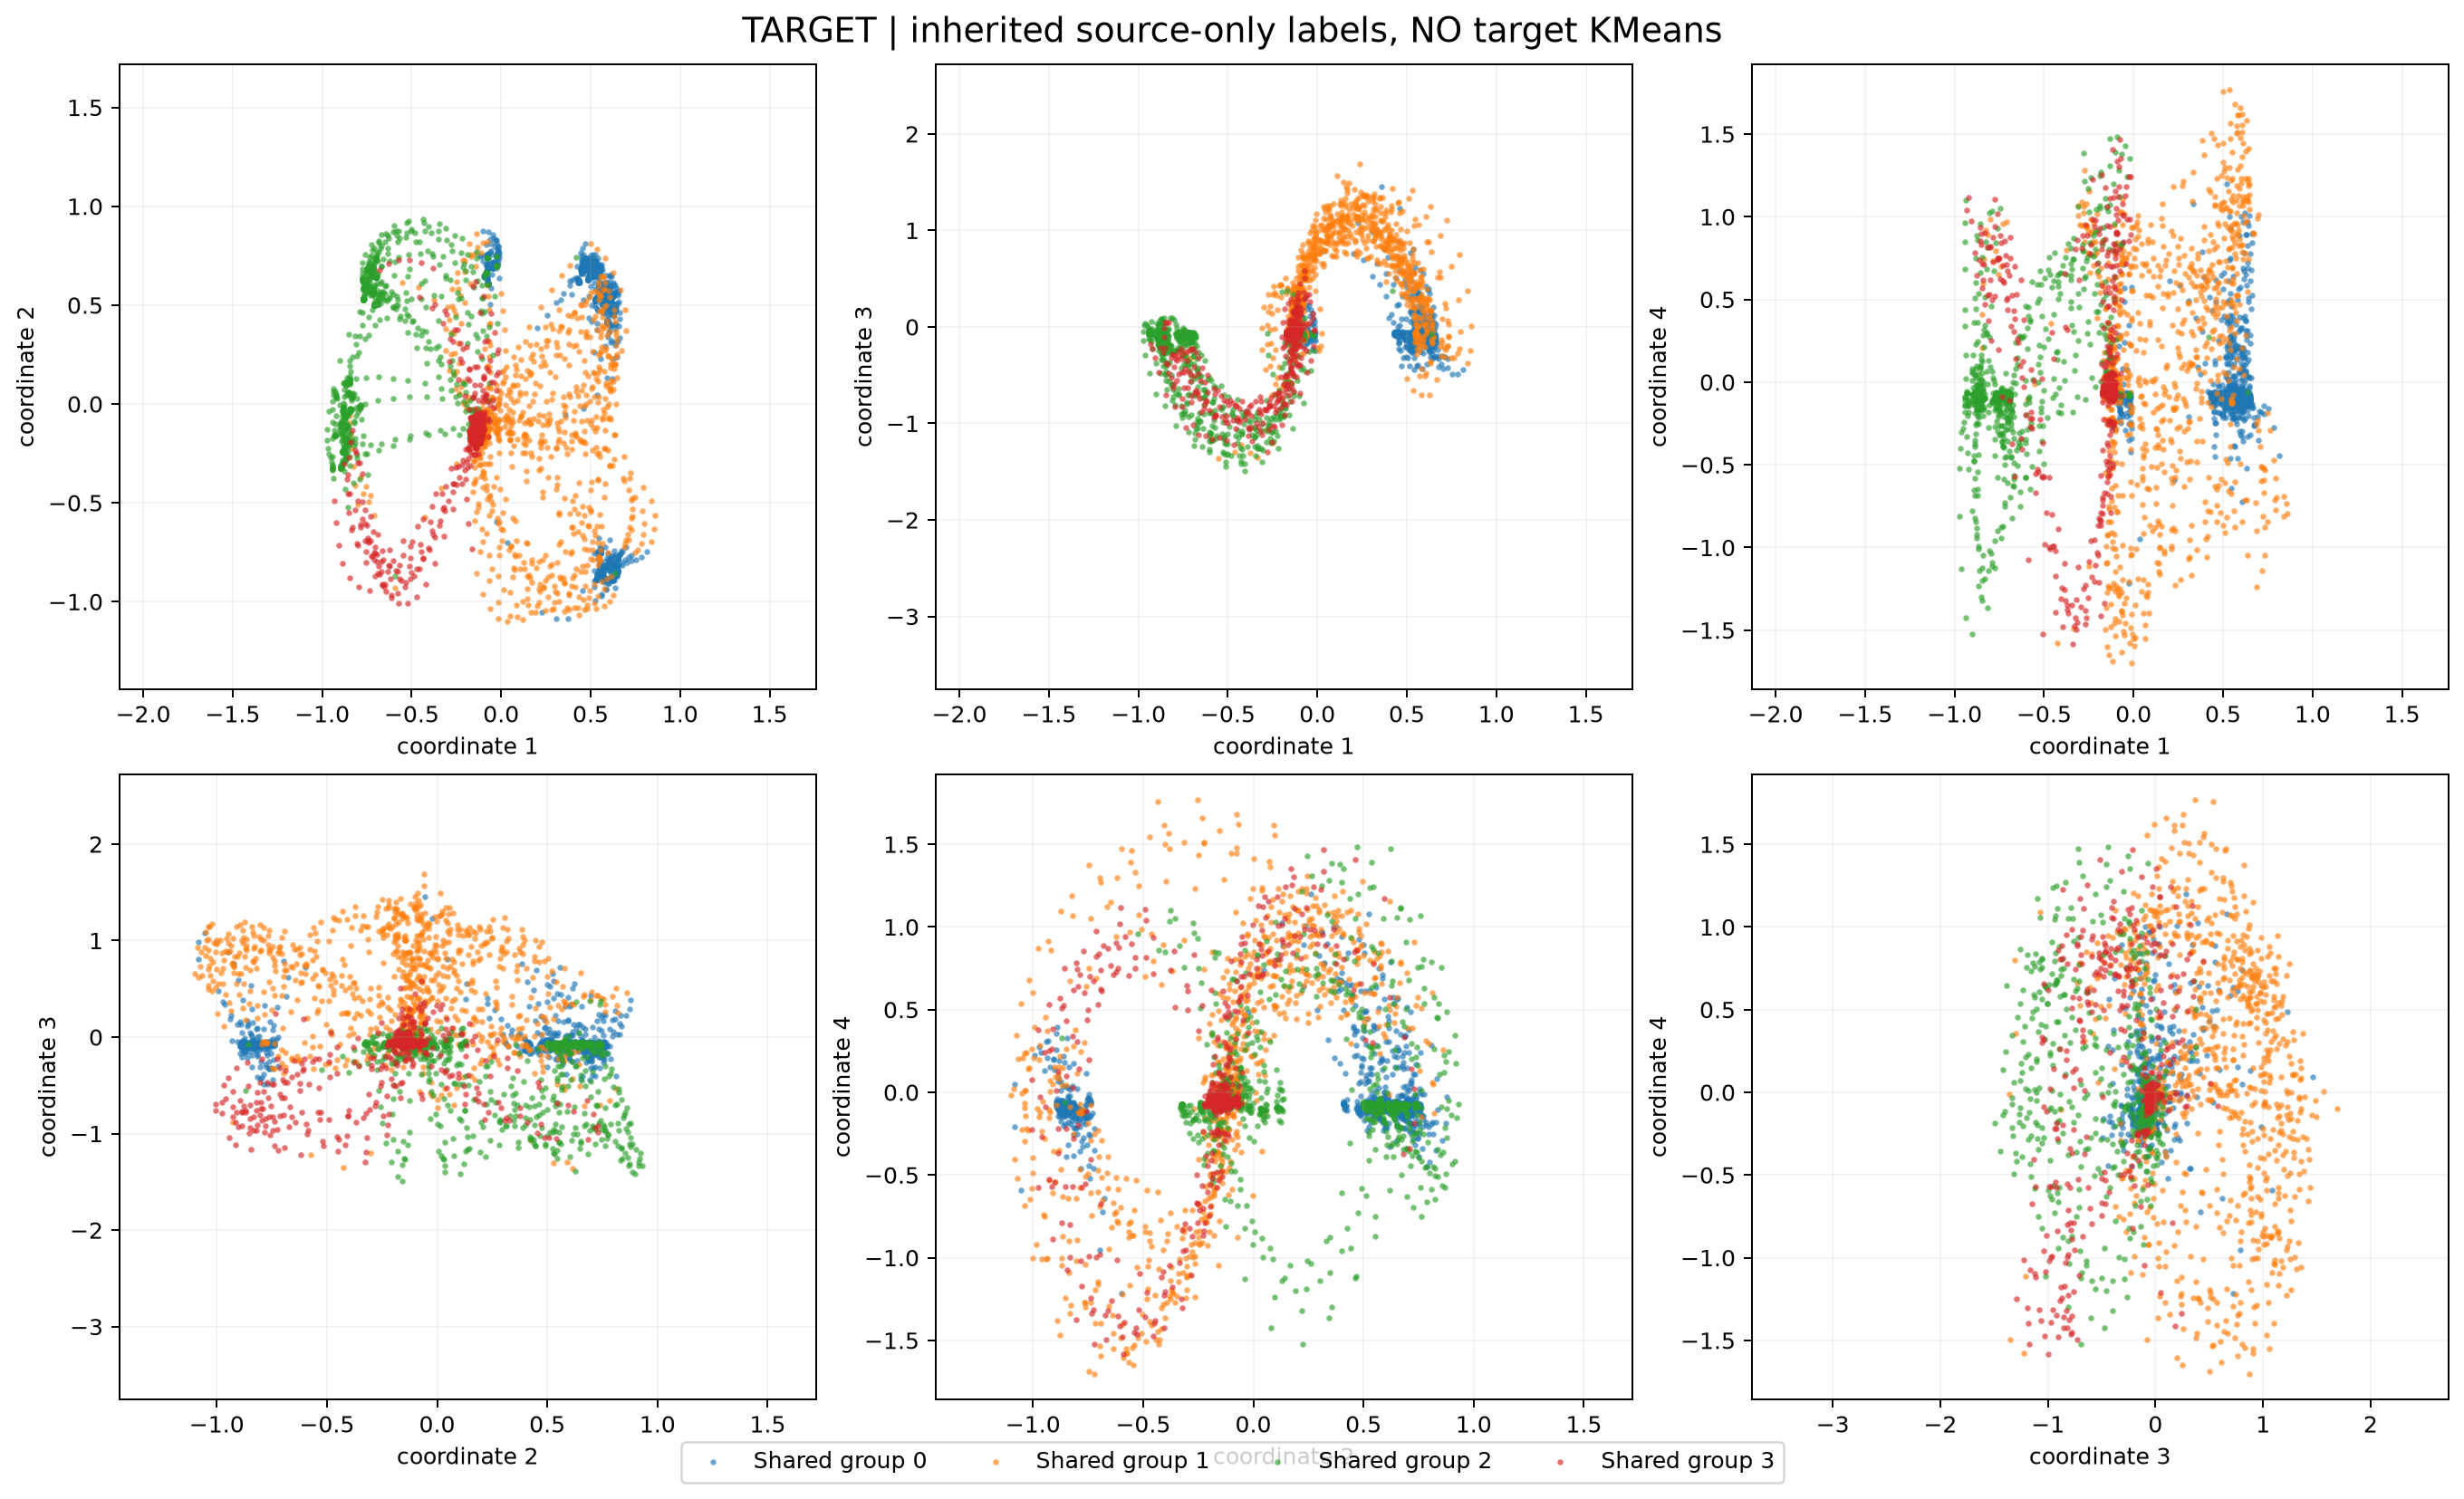
\includegraphics[width=\textwidth]{target_shared_test_six.png}
\caption{原始目标域：颜色完全继承配对源域，没有目标域聚类。}
\end{figure}
\clearpage
\begin{figure}[p]\centering
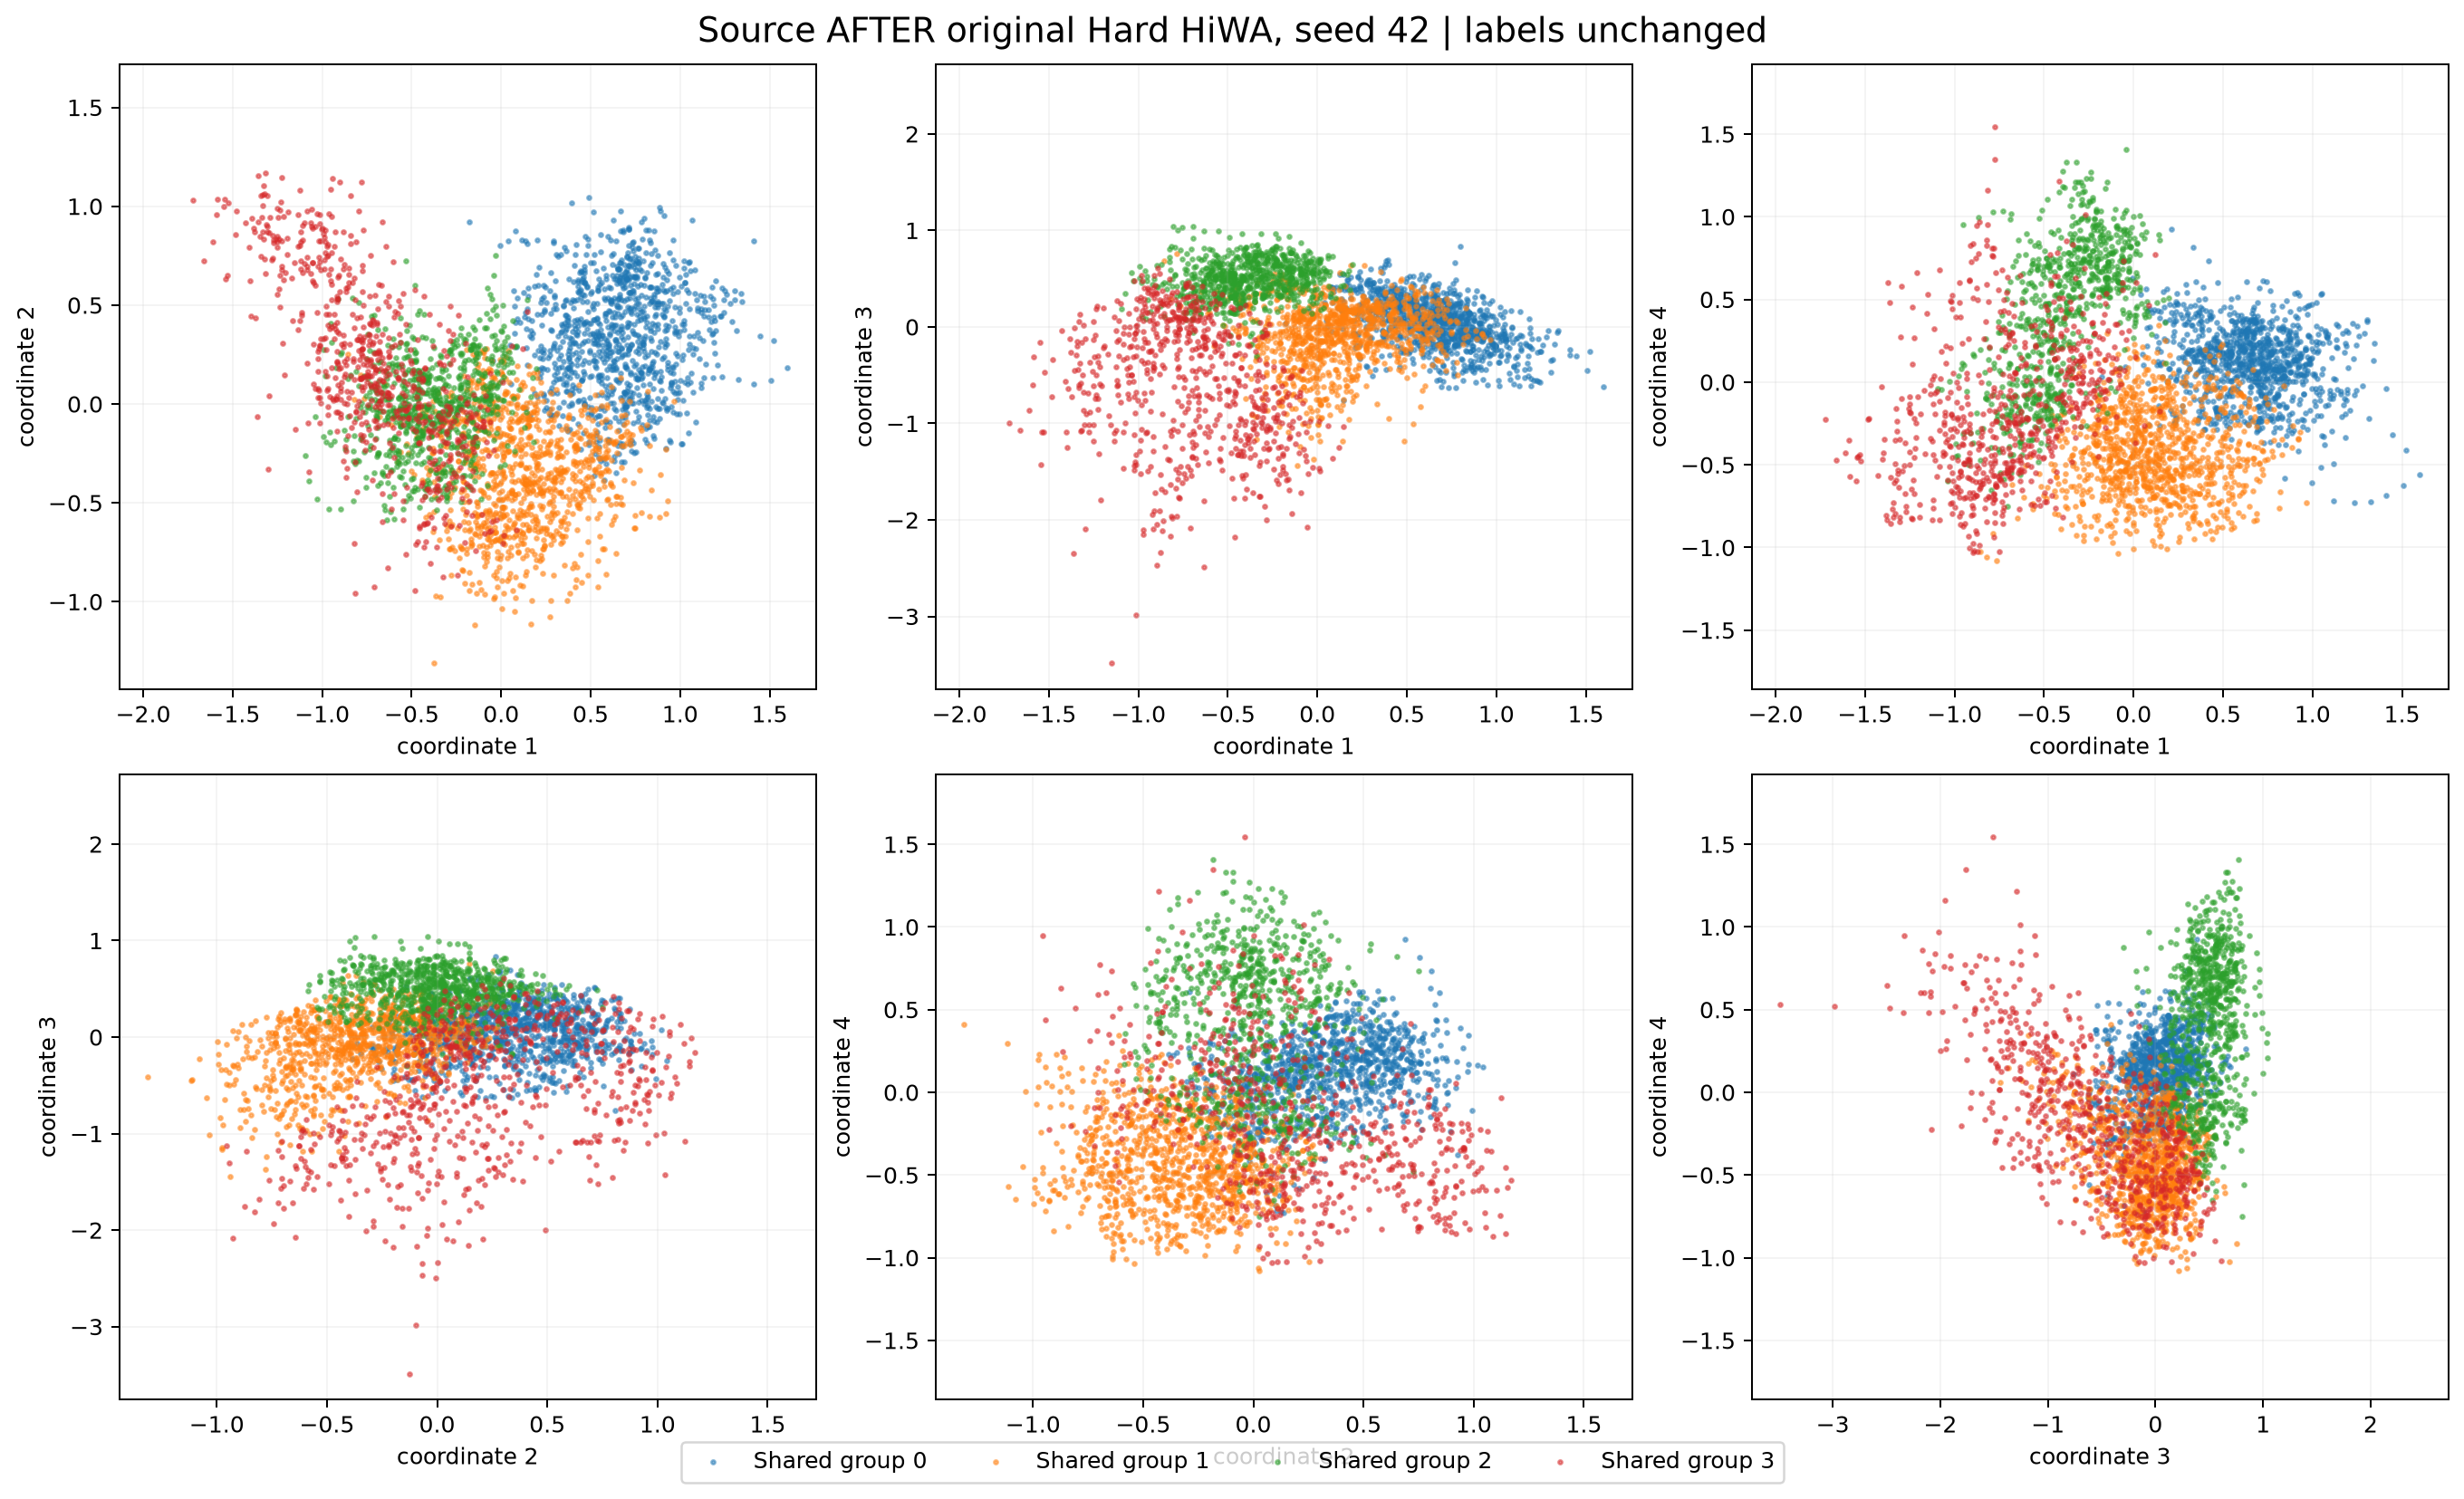
\includegraphics[width=\textwidth]{source_after_test_six.png}
\caption{原版 Hard HiWA 正交变换后的源域（seed 42）：颜色完全不改变。}
\end{figure}
\clearpage
\begin{figure}[p]\centering
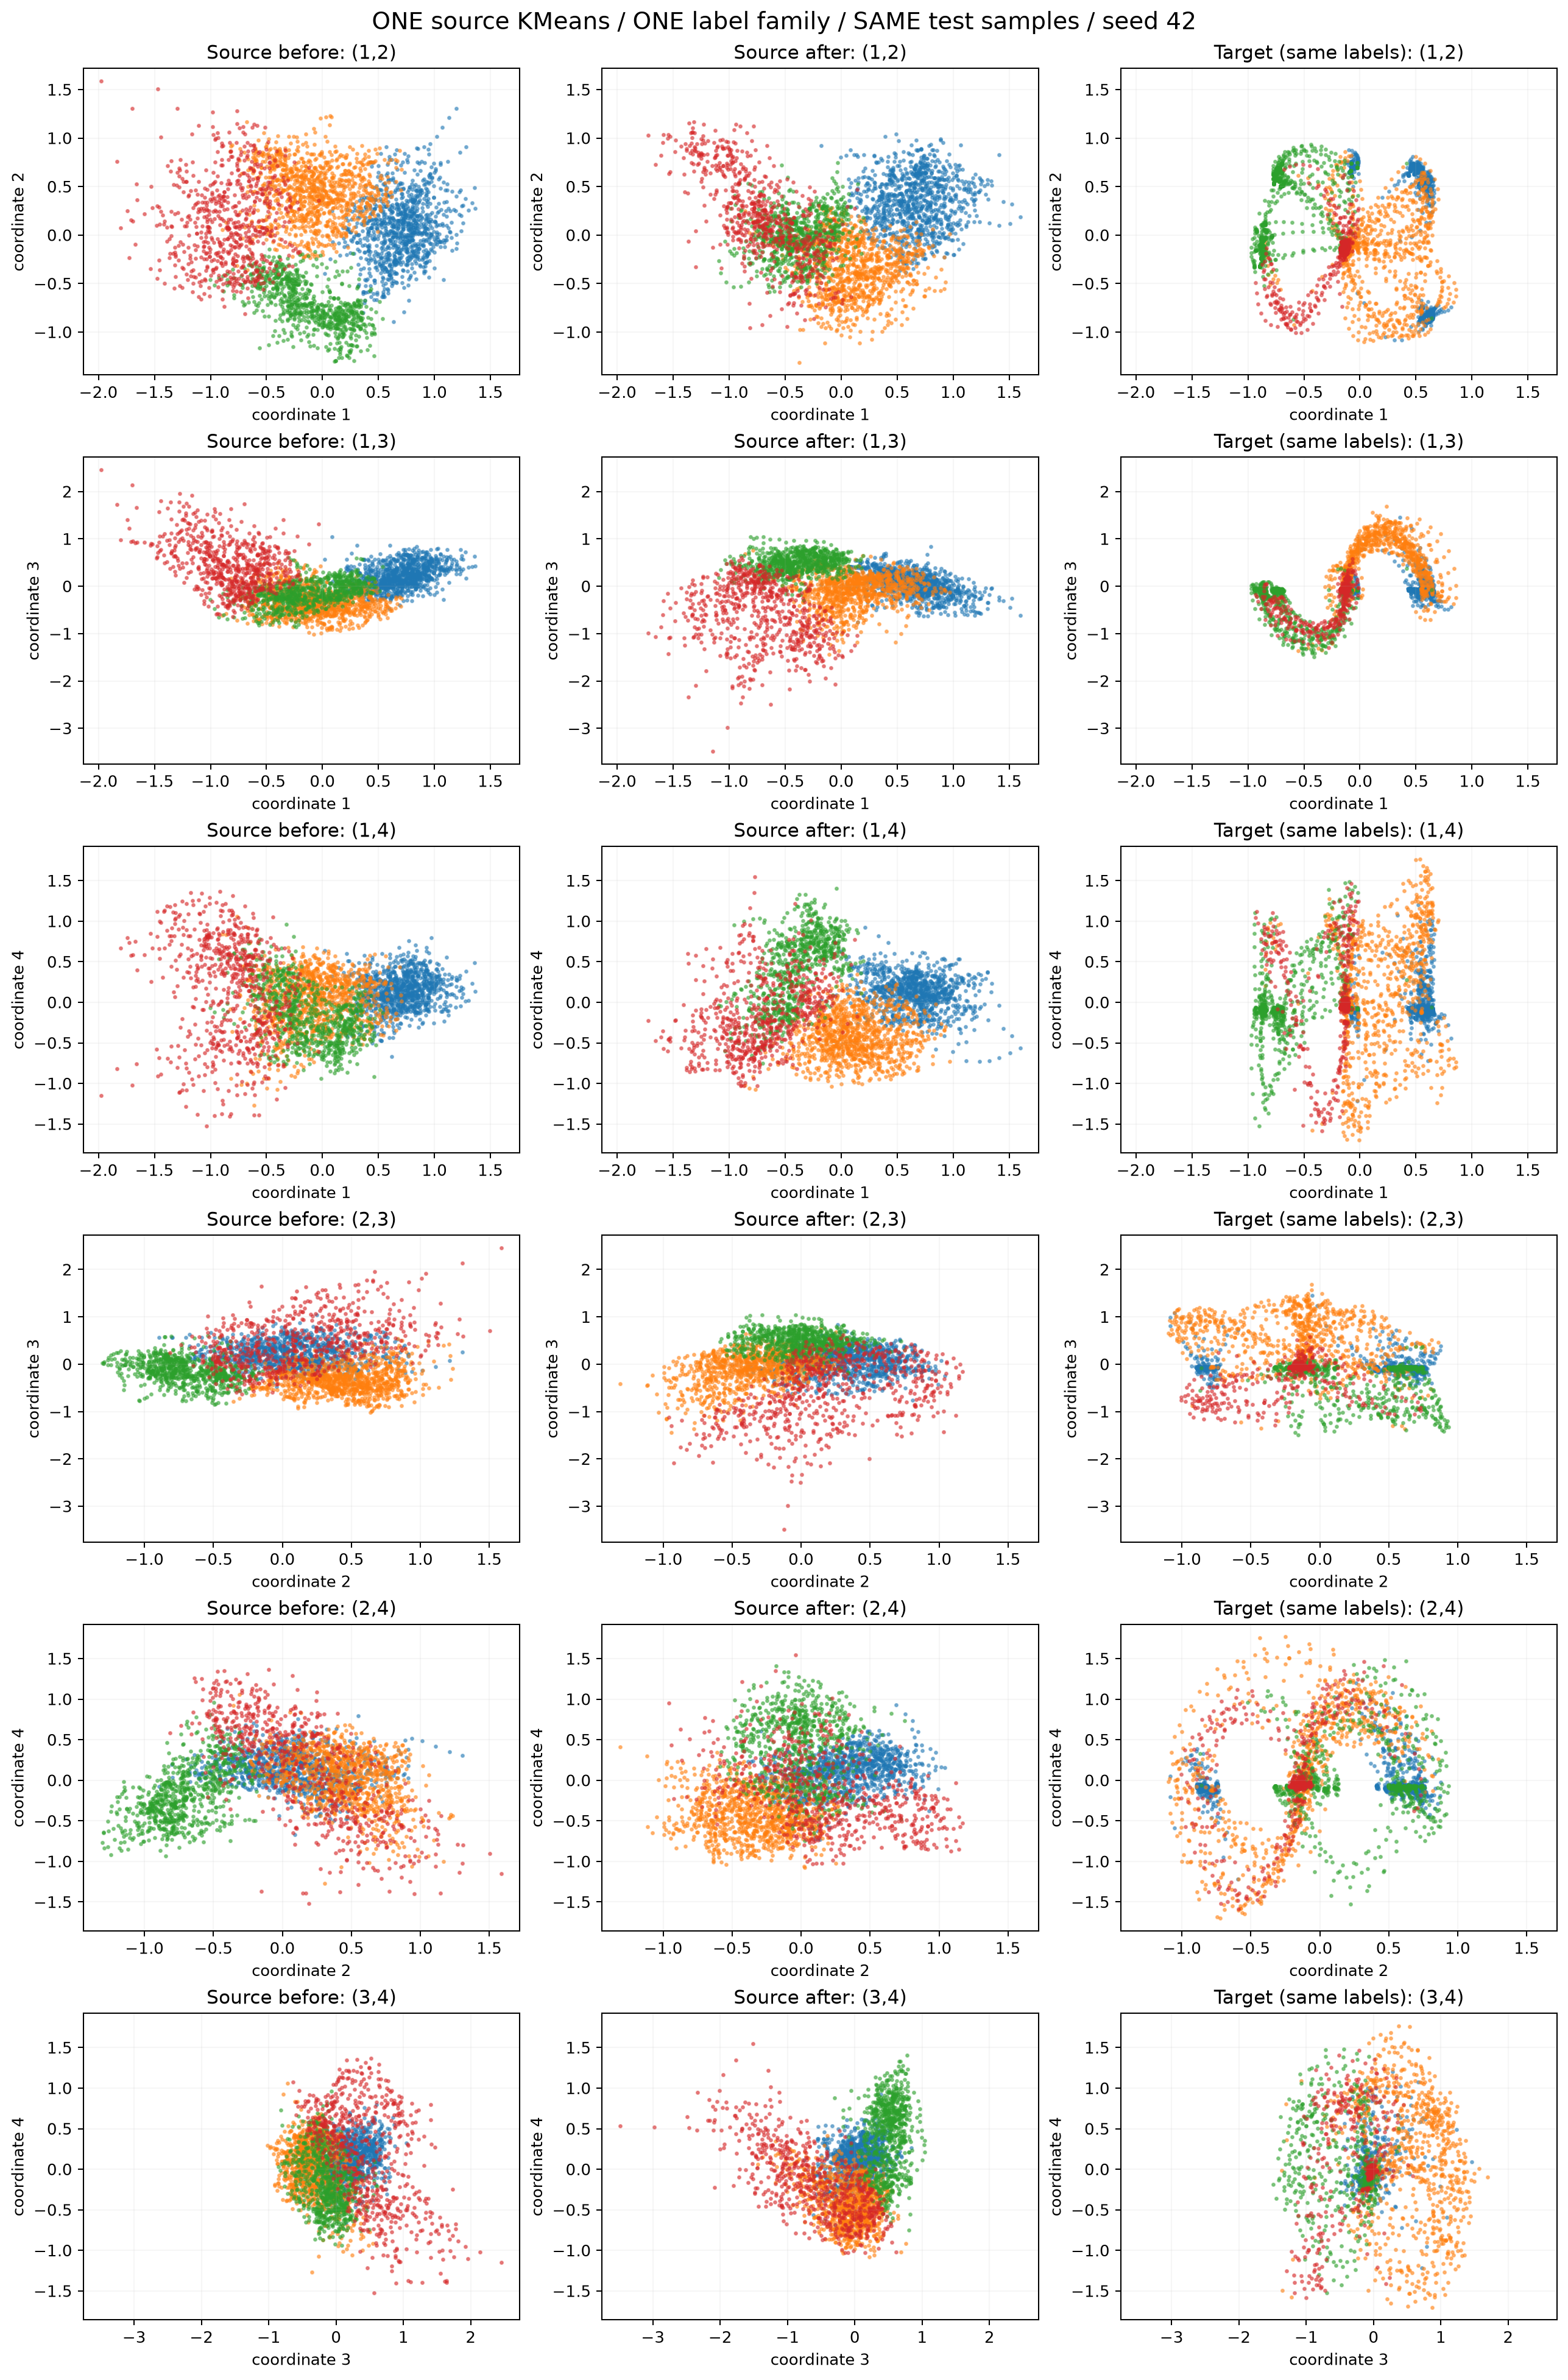
\includegraphics[width=\textwidth,height=.86\textheight,keepaspectratio]
{before_after_target_six_pairs.png}
\caption{逐投影三列直接对照：源域原始、源域旋转后、目标域；
相同样本、相同颜色、相同轴范围。所有行的颜色固定来源于源域一次 K-means。}
\end{figure}
\clearpage

\section{同一口径的实际评价}
全部在留出测试数据上评估。记源域为归一化 $x_i$、目标为 $y_i$、
估计正交矩阵为 $\widehat R$。
\begin{align}
 \mathrm{MAE}&=\frac1{4N}\sum_{i=1}^N\sum_{j=1}^4
      |(\widehat Rx_i)_j-(y_i)_j|,\\
 \mathrm{paired\!-\!rMSE}&=
      \frac{\sum_i\|\widehat R x_i-y_i\|_2^2}
           {\sum_i\|y_i\|_2^2},\\
 R^2&=1-\frac{\sum_i\|\widehat Rx_i-y_i\|_2^2}
                 {\sum_i\|y_i-\bar y\|_2^2}.
\end{align}
本文的 1NN 按压缩包评估程序的查询方向：每个目标测试点 $y_i$
查询最近的对齐源测试点 $\widehat R x_{j(i)}$，再比较两者的
\emph{共同标签}：
\begin{equation}
 1\mathrm{NN}=\frac1N\sum_i
 \mathbf1\{c_{j(i)}=c_i\},\quad
 j(i)=\arg\min_j\|y_i-\widehat Rx_j\|_2.
\end{equation}
\textbf{目标标签继承自真实配对，因此 1NN 是固定标签邻域保留率，
不是独立的真实运动类别识别准确率。}

另外报告作者原版旋转 rMSE 的\emph{代理值}：
\begin{equation}
 \mathrm{rMSE}_{\mathrm{proxy}}=
 \frac{\|R_{\mathrm{ref}}X^\top-\widehat RX^\top\|_F^2}
      {\|R_{\mathrm{ref}}X^\top\|_F^2},
\end{equation}
其中 $R_{\mathrm{ref}}$ 是\emph{仅用训练集同步配对}拟合的正交
Procrustes，而非不存在的真实旋转 $R_{\mathrm{gt}}$。
不能将该代理值冒充真实作者 rMSE。原版求解器的
\texttt{\_eval\_R2} 不采用标准平方残差，
我们在独立评价器中计算标准 $R^2$，不修改原版求解器。

\begin{table}[H]\centering\small
\caption{真实重做实验，留出测试集指标。MAE 与 rMSE 为无量纲归一化数据上的值。}
\resizebox{\textwidth}{!}{%
\begin{tabular}{lrrrrr}\toprule
方法 & 共享标签 1NN $\uparrow$ & MAE $\downarrow$ &
paired-rMSE $\downarrow$ & 旋转 rMSE 代理 $\downarrow$ & $R^2 \uparrow$\\\midrule
\primitiveinput{results/source_only_fixed_groups/metrics_rows.tex}
\bottomrule
\end{tabular}}
\end{table}
\begin{figure}[H]\centering
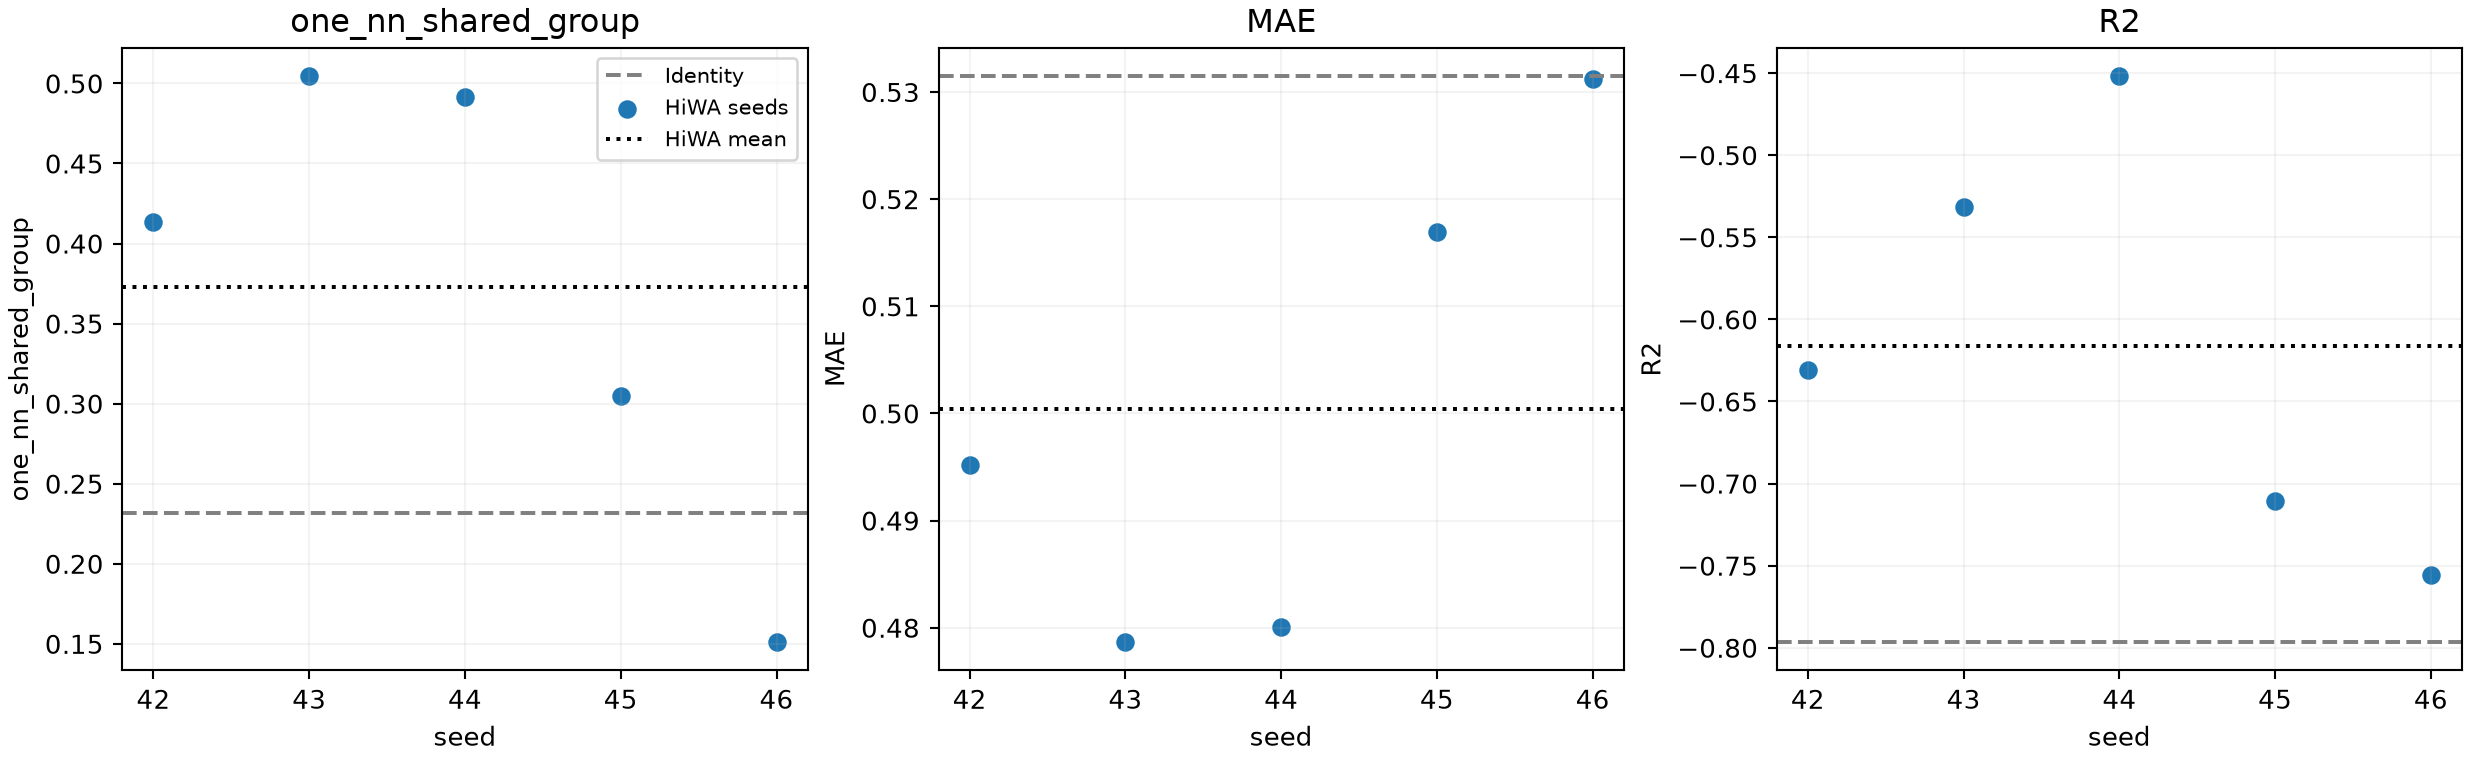
\includegraphics[width=\textwidth]{frozen_label_metrics.png}
\caption{五个种子与未对齐基线：1NN、MAE、标准 $R^2$。}
\end{figure}

\section{解释范围、文件与可复现性}
主结论只由本次同一标签协议的真实数值支持，
不能用先前独立聚类协议的 $R^2$ 或 1NN 数值替代。
尤其是统一标签本身利用了真实同步配对，不意味着方法自动从
完全无标签目标域恢复了组语义。

复现输入：\texttt{results/clustering/clustered\_4d.npz}
（只复用其 4D 特征与 train/test 标记，丢弃旧簇标签）。
复现代码：
\texttt{code/source\_only\_fixed\_group\_pipeline.py}
$\to$ \texttt{code/run\_hard\_hiwa.py}
$\to$ \texttt{code/evaluate\_fixed\_group\_alignment.py}；
数值报告：
\texttt{results/source\_only\_fixed\_groups/RUN\_REPORT.md}。
所有原始旋转矩阵、簇传输矩阵、数值审计结果与图表均保留在
\texttt{results/source\_only\_fixed\_groups/}。

\end{document}
